\chapter{Introduction}
\label{sec:Introduction}
Carbon-Hydrogen (C-H) bonds are one of the most stable bonds in nature, making them generally unreactive. On the one hand this is great, as all organic molecules, are based on a backbone of carbon atoms, each typically bonded to hydrogen atoms. That means that hydrocarbons and biomolecules stay intact under normal conditions, so that our body, fuels and plastics do not spontaneously fall apart. On the other side this stability can be a challenge for synthetic chemistry if these bonds need be modified. This is where the field of C-H activation is working on. \\\\ 
\textbf{But why is this relevant?} \\ \\
C-H activation has the potential to revolutionize the chemical industry. Alkanes, or saturated hydrocarbons, are major constituents of natural gas \cite{labinger2002understanding}, which is a large and low-cost feedstock which remains unused for chemical synthesis \cite{bergman2007c} due to their chemical inertness. Until know, there are very few practical processes for converting them directly to more valuable products. Alkanes react at high temperatures, as in a combustion engine, however these reactions only yield the unattractive products carbon dioxide and water. Selective C-H activation and transformation of such unsaturated hydrocarbons offers a power strategy to place chemical groups directly at a desired part in a molecule. Traditional synthetic approaches, like cross-couplings reactions (recognized with the 2010 Noble price in Chemistry) \cite{Nobleprice2010, suzuki2011noble, negishi2011nobleprice}, require multiple steps and pre-functionalization to achieve comparable results. By bypassing pre-functionalization, selective C-H activation not only streamlines synthesis, but also reduces the generation of hazardous waste \cite{rogge2021c, goldberg2017large}, aligning with the principles of green chemistry \cite{dalton2021c}. \\ \\
\textbf{So how can C-H bonds be activated?} \\ \\
One approach to activating C-H bonds is using transition metal complexes. Typically these reactions are conducted at high temperatures or in a special solvent, as they require the dissociation of one ligand to form a highly reactive 16 valence electron species. A more energy sustainable approach would be to form the reactive species photo chemically \cite{arndtsen1995selective, Hartwig_book}, which can be achieved at room temperature. The open coordination site of the low valent metal complex enables the binding of an alkane \cite{hall1992matrix, jones2003isotope, crabtree1988hh, altus2021continuum} and subsequently, the activation of one it's C-H bonds \cite{hammarback2021direct, lian1996femtosecond, bromberg1996ultrafast, bromberg1997mechanism}. The key intermediate in these photochemical C-H activation reactions are so-called $\sigma$-alkane complexes, in which a C-H bond loosely binds to the metal (see schematic in Figure \ref{fig:scheme_photochem_C_H}).
\begin{figure}[H]
    \centering
    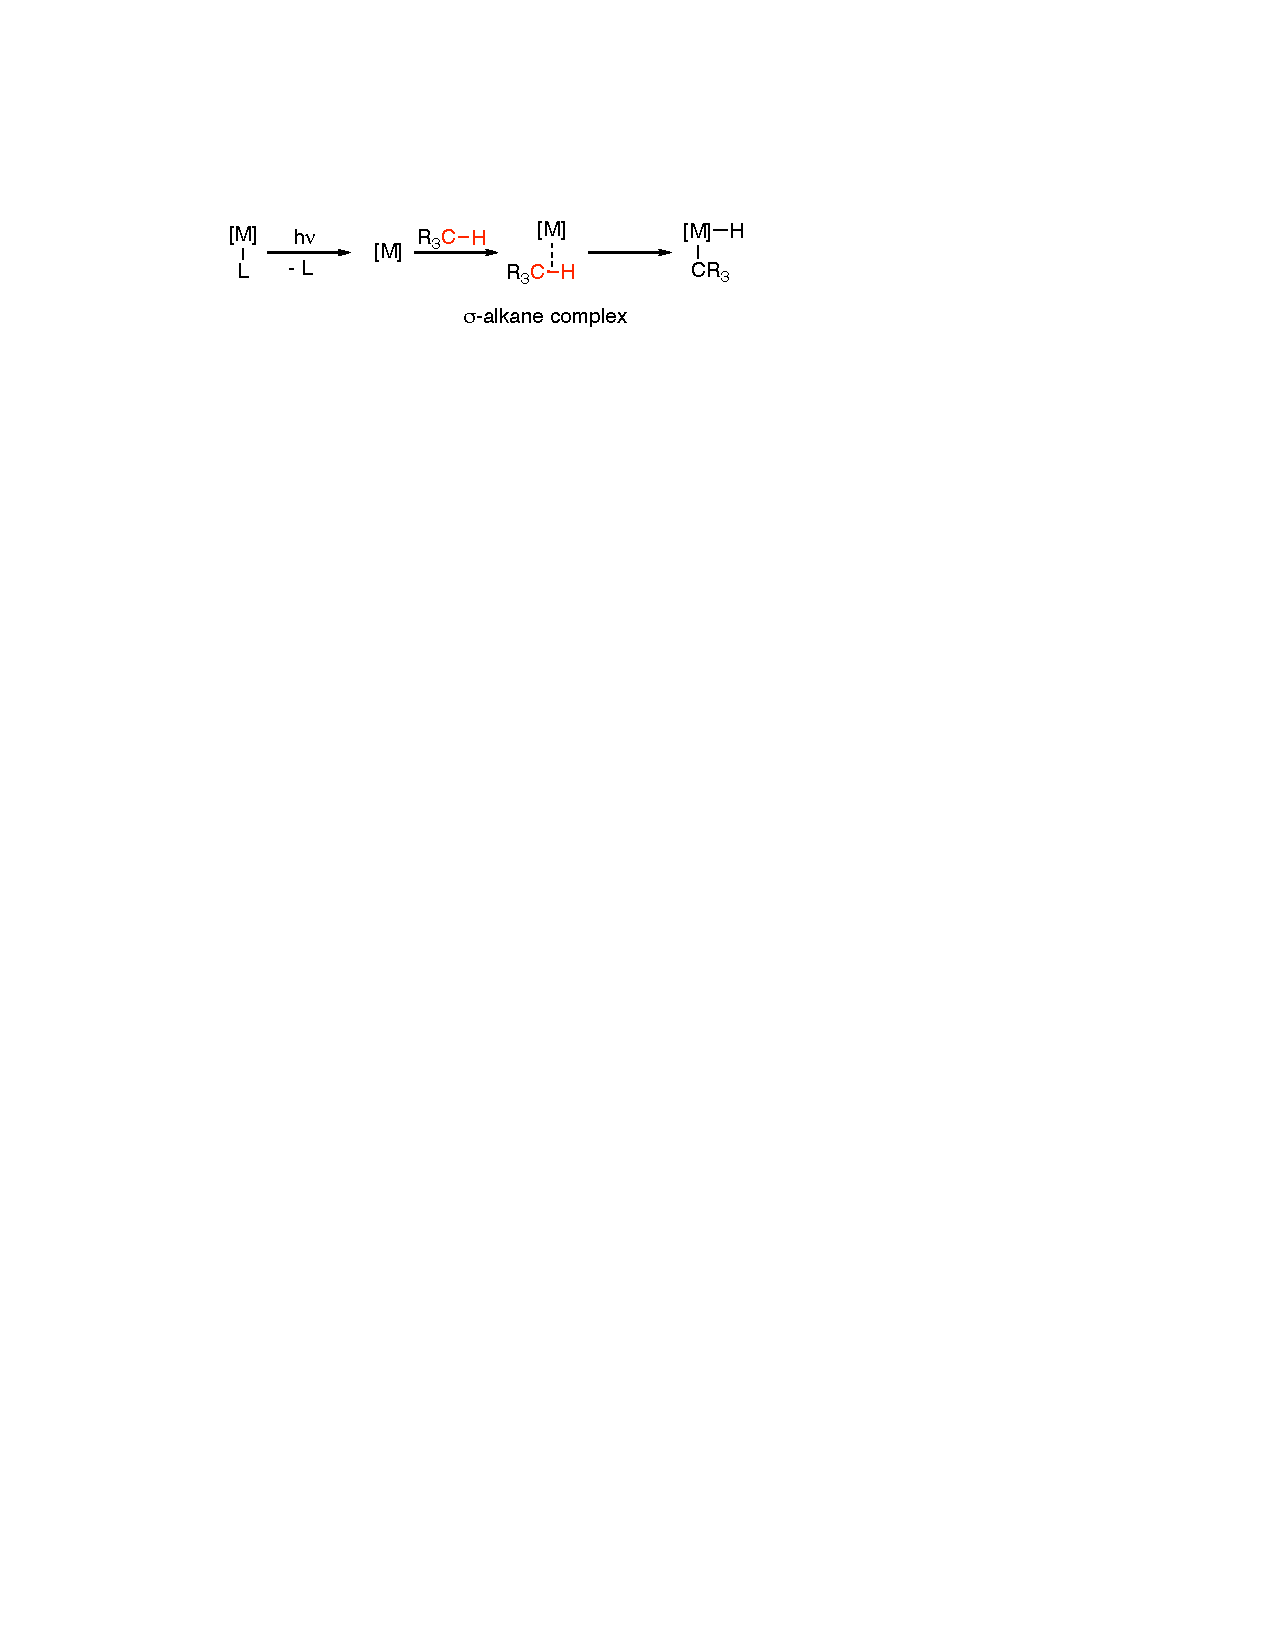
\includegraphics[width=0.8\linewidth]{Figures/Transition_Metal_Catalysis.pdf}
    \caption{Schematic for photochemical C-H activation. [M] is an example metal complex where a ligand L can be photochemically cleaved.}
    \label{fig:scheme_photochem_C_H}
\end{figure}
\noindent
$\sigma$-alkane complexes are short-lived, typically exhibiting lifetimes on the picosecond (ps) timescale. Their electronic properties play a key role in determining whether a metal complex is suitable for C-H activation: The reaction may proceed via oxidative addition, in which the metal is inserted into the C-H bond, or it may terminate at the formation of the $\sigma$-alkane complex. Consequently, probing these short-lived intermediates is essential for understanding what determines reactivity of a given transition metal complex. 
\\ \\ \textbf{How can $\sigma$-alkane complexes be probed?} \\ \\
Conventional approaches methods like isotope labeling \cite{jones2003isotope} and nuclear magnetic resonance (NMR) spectroscopy \cite{ball2007delicate, bernskoetter2009characterization, watson2022binding} have been instrumental in revealing the overall mechanisms in C-H activation. Neutron and X-ray diffraction \cite{pike2015solid, chadwick2016selective, evans1997heptane, gyton2025operationally} are decisive for determining the structures of frozen or crystallized $\sigma$-alkane complexes. Time-resolved infrared (IR) spectroscopy has proven essential for detecting and structurally characterizing short-lived intermediates during the reaction pathway \cite{bromberg1997mechanism, lian1996femtosecond, bengali1994activation, schultz1994ir, fairlamb2024unveiling}. However, all these techniques lack the sensitivity to directly probe electronic structure which limits their ability to correlate the underlying electronic interactions with C-H bond reactivity. This were time-resolved X-ray absorption spectroscopy (XAS) and resonant inelastic X-ray scattering (RIXS), which are the main two techniques of this thesis, can be utilized to fill this information gap.\\ \\
In the following chapters will go into more detail about the background of the electronic structure of transition metal complexes during photochemical C-H activation (Chapter \ref{chapter:background}) and will have a more detailed look at the methods used in this thesis (Chapter \ref{chapter:X-ray_Based_Spectroscopy_Methods}). \textcolor{red}{ADD PART about the Papers}

